数字电路一般可分为\textbf{{组合逻辑电路和时序逻辑电路。}}

\textbf{组合逻辑电路}在逻辑功能上的特点是任意时刻的输出\textbf{仅仅取决于该时刻的输入,}与电路原来的状态无关。也就是说,组合逻辑电路没有``记忆'',运算后的结果要立刻送入寄存器保存。

\textbf{时序逻辑电路}在逻辑功能上的特点是任意时刻的输出\textbf{不仅取决于当时的输入信号,还取决于电路原来的状态}。也就是说,时序逻辑电路具有记忆元件,即触发器(能够存储一位信号的基本单元电路),可以记录前一时刻的输出状态(CPU就是一种复杂的时序逻辑电路)。

ALU是一种\textbf{组合逻辑电路},因此在实际使用ALU时,其输入端口A和B必须与锁存器相连,而且在运算的过程中锁存器的内容是不变的,其输出也必须送至寄存器保存。

\textbf{{ALU的主要功能:}}ALU的功能不仅是执行各种算术(加、减、乘、除)和逻辑运算(``与''、``或''、``非''、``异或''等)操作的部件,还具有先行进位逻辑。其实在并行加法器之并行进位链里面就使用了ALU,只是当时还没有介绍ALU的概念,下面将会和前面的内容联系起来讲解。

ALU的电路框架如下图所示。

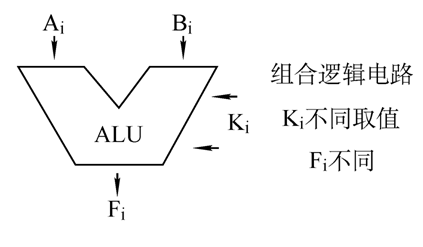
\includegraphics[width=1.87500in,height=1.09375in]{png-jpeg-pics/CFF08CB305A273F5164B115D7CDD5139.png}
